\section{Orthogonal projections and Fourier series}

We now reconsider a problem that we briefly encountered, only in the
context of $\R^3$, in Section~\ref{sec:planes}: how to find the
shortest distance between a point and a subspace. The method we used
in Section~\ref{sec:planes} (see
Example~\ref{exa:shortest-distance-plane}) relies on the existence of
normal vectors and does not generalize beyond $\R^3$. The following
proposition gives a much better method for solving this problem,
provided that we have an orthogonal basis of the subspace.

\begin{proposition}{Orthogonal projection onto a subspace}{projection-subspace}
  Let $V$ be an inner product space, and let $W$ be a subspace of
  $V$. Assume $\set{\vect{u}_1,\ldots,\vect{u}_k}$ is an orthogonal
  basis of\/ $W$, and $\vect{v}\in V$ is any vector. Then the
  following vector $\vect{v}'$ is the element of $W$ that is closest
  to $\vect{v}$, i.e., such that $\norm{\vect{v}-\vect{v}'}$ is as
  small as possible.
  \begin{equation*}
    \vect{v}' =
    \frac{\iprod{\vect{v},\vect{u}_1}}{\iprod{\vect{u}_1,\vect{u}_1}}\,\vect{u}_1
    + \frac{\iprod{\vect{v},\vect{u}_2}}{\iprod{\vect{u}_2,\vect{u}_2}}\,\vect{u}_2
    + \ldots
    + \frac{\iprod{\vect{v},\vect{u}_k}}{\iprod{\vect{u}_k,\vect{u}_k}}\,\vect{u}_k.
  \end{equation*}
  Moreover, the vector $\vect{v}-\vect{v}'$ is orthogonal to $W$.
  \begin{center}
    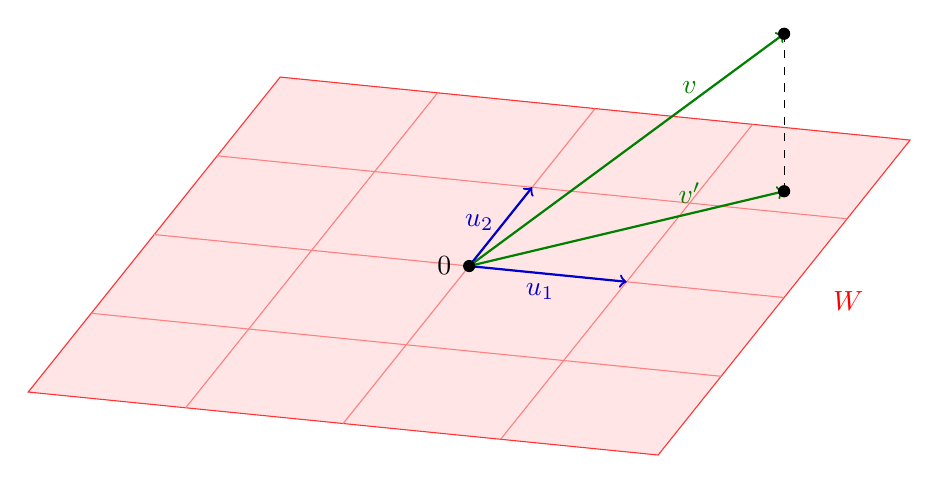
\begin{tikzpicture}[x={(1cm,-0.1cm)},y={(0.4cm,0.5cm)},z={(0cm,1cm)}]
      \filldraw[draw=red!80,fill=red!10](-4,-4,0) -- (4,-4,0) -- (4,4,0) -- (-4,4,0) -- cycle;
      \path[red] (4.5,0,0) node[right] {$W$};
      \draw[thin,red!50] (-2,-4,0) -- (-2,4,0);
      \draw[thin,red!50] (0,-4,0) -- (0,4,0);
      \draw[thin,red!50] (2,-4,0) -- (2,4,0);
      \draw[thin,red!50] (-4,-2,0) -- (4,-2,0);
      \draw[thin,red!50] (-4,0,0) -- (4,0,0);
      \draw[thin,red!50] (-4,2,0) -- (4,2,0);
      \draw[->,thick,blue!80!black](0,0,0) -- node[below, pos=0.45]{$\vect{u}_1$} (2,0,0);
      \draw[->,thick,blue!80!black](0,0,0) -- node[left, pos=0.55]{$\vect{u}_2$} (0,2,0);
      \draw[->,thick,green!50!black](0,0,0) -- node[above, pos=0.7] {$\vect{v}$} (3,2.5,2);
      \draw[->,thick,green!50!black](0,0,0) -- node[above, pos=0.7] {$\vect{v}'$} (3,2.5,0);
      \draw[dashed](3,2.5,0) -- (3,2.5,2);
      \fill (0,0,0) circle [radius=2.2pt] node [left=3pt] {$\vect{0}$};
      \fill (3,2.5,2) circle [radius=2.2pt];
      \fill (3,2.5,0) circle [radius=2.2pt];
    \end{tikzpicture}
  \end{center}
  The vector $\vect{v}'$ is called the \textbf{orthogonal projection
    of $\vect{v}$ onto $W$}%
  \index{orthogonal projection!onto subspace}%
  \index{projection!onto subspace}.
\end{proposition}

\begin{proof}
  Since $\set{\vect{u}_1,\ldots,\vect{u}_k}$ is a basis of $W$, every
  vector $\vect{w}\in W$ is of the form
  $\vect{w} = x_1\vect{u}_1 + \ldots + x_k\vect{u}_k$, where
  $x_1,\ldots,x_k\in\R$. We have
  \begin{eqnarray*}
    \norm{\vect{v}-\vect{w}}^2
    &=& \iprod{\vect{v}-\vect{w}, \vect{v}-\vect{w}} \\
    &=& \iprod{\vect{v}, \vect{v}} - 2\iprod{\vect{v},\vect{w}} + \iprod{\vect{w},\vect{w}} \\
    &=& \iprod{\vect{v}, \vect{v}} - 2\iprod{\vect{v},x_1\vect{u}_1 + \ldots + x_k\vect{u}_k} + \iprod{x_1\vect{u}_1 + \ldots + x_k\vect{u}_k, x_1\vect{u}_1 + \ldots + x_k\vect{u}_k} \\
    &=& \iprod{\vect{v}, \vect{v}} - 2x_1\iprod{\vect{v},\vect{u}_1} - \ldots - 2x_k\iprod{\vect{v},\vect{u}_k} + x_1^2\iprod{\vect{u}_1, \vect{u}_1} + \ldots + x_k^2\iprod{\vect{u}_k, \vect{u}_k} \\
    &=& \iprod{\vect{v}, \vect{v}} + (x_1^2\iprod{\vect{u}_1, \vect{u}_1} - 2x_1\iprod{\vect{v},\vect{u}_1}) + \ldots + (x_k^2\iprod{\vect{u}_k, \vect{u}_k} - 2x_k\iprod{\vect{v},\vect{u}_k}).
  \end{eqnarray*}
  Here, in the second-to-last step, we have used the fact that
  $\iprod{\vect{u}_i,\vect{u}_j}=0$ when $i\neq j$, i.e., the
  orthogonality of $\vect{u}_1,\ldots,\vect{u}_k$.  Therefore, the
  expression $\norm{\vect{v}-\vect{w}}^2$ is minimized when each of the
  expressions
  \begin{equation}\label{eqn:projection-subspace}
    x_1^2\iprod{\vect{u}_1, \vect{u}_1} - 2x_1\iprod{\vect{v},\vect{u}_1}, \qquad
    \ldots,\qquad
    x_k^2\iprod{\vect{u}_k, \vect{u}_k} - 2x_k\iprod{\vect{v},\vect{u}_k}
  \end{equation}
  takes its minimum. By the laws of calculus, the minimum of a
  function of the form $f(x)=ax^2-2bx$ occurs when $f'(x)=2ax-2b=0$,
  i.e., when $x=\frac{b}{a}$. Applying this reasoning to each of the
  $k$ expressions in {\eqref{eqn:projection-subspace}}, we find that the
  minimum occurs when
  \begin{equation*}
    x_1 = \frac{\iprod{\vect{v},\vect{u}_1}}{\iprod{\vect{u}_1,\vect{u}_1}},\quad
    \ldots,\quad
    x_k = \frac{\iprod{\vect{v},\vect{u}_k}}{\iprod{\vect{u}_k,\vect{u}_k}},
  \end{equation*}
  i.e., when
  \begin{equation*}
    \vect{w} =
    \frac{\iprod{\vect{v},\vect{u}_1}}{\iprod{\vect{u}_1,\vect{u}_1}}\,\vect{u}_1
    + \frac{\iprod{\vect{v},\vect{u}_2}}{\iprod{\vect{u}_2,\vect{u}_2}}\,\vect{u}_2
    + \ldots
    + \frac{\iprod{\vect{v},\vect{u}_k}}{\iprod{\vect{u}_k,\vect{u}_k}}\,\vect{u}_k.
  \end{equation*}
  This is what had to be shown. Finally, to show that
  $\vect{v}-\vect{v}'$ is orthogonal to $W$, it suffices to show that
  $\vect{v}-\vect{v}'$ is orthogonal to each basis vector
  $\vect{u}_1,\ldots,\vect{u}_k$ of $W$. We show this by direct calculation.
  Consider $i\in\set{1,\ldots,k}$. First note that
  \begin{eqnarray*}
    \iprod{\vect{v}',\vect{u}_i}
    &=& \bigiprod{\paren{
        \frac{\iprod{\vect{v},\vect{u}_1}}{\iprod{\vect{u}_1,\vect{u}_1}}\,\vect{u}_1
        + \ldots
        + \frac{\iprod{\vect{v},\vect{u}_k}}{\iprod{\vect{u}_k,\vect{u}_k}}\,\vect{u}_k}
        ,\vect{u}_i}\\
    &=&
        \frac{\iprod{\vect{v},\vect{u}_1}}{\iprod{\vect{u}_1,\vect{u}_1}}\,\iprod{\vect{u}_1,\vect{u}_i}
        + \ldots
        + \frac{\iprod{\vect{v},\vect{u}_k}}{\iprod{\vect{u}_k,\vect{u}_k}}\,\iprod{\vect{u}_k,\vect{u}_i}
    \\
    &=& \frac{\iprod{\vect{v},\vect{u}_i}}{\iprod{\vect{u}_i,\vect{u}_i}}\,\iprod{\vect{u}_i,\vect{u}_i}\\
    &=& \iprod{\vect{v},\vect{u}_i}.
  \end{eqnarray*}
  Therefore,
  $\iprod{\vect{v}-\vect{v}',\vect{u}_i} = \iprod{\vect{v},\vect{u}_i}
  - \iprod{\vect{v}',\vect{u}_i} = 0$, and $\vect{v}-\vect{v}'$ is
  orthogonal to $\vect{u}_i$, as desired.
\end{proof}

\begin{example}{Orthogonal projection onto a subspace}{projection-subspace}
  Consider $\R^4$ with the usual dot product. Let
  $W=\sspan\set{\vect{u}_1,\vect{u}_2}$, where
  \begin{equation*}
    \vect{u}_1 = \begin{mymatrix}{r} 1 \\ 1 \\ 2 \\ 0 \end{mymatrix}, \quad
    \vect{u}_2 = \begin{mymatrix}{r} -1 \\ -1 \\ 1 \\ 3 \end{mymatrix}.
  \end{equation*}
  Note that $\vect{u}_1$ and $\vect{u}_2$ are orthogonal. Let
  \begin{equation*}
    \vect{v} = \begin{mymatrix}{r} 1 \\ 2 \\ 3 \\ 4 \end{mymatrix}.
  \end{equation*}
  Find the element of\/ $W$ that is closest to $\vect{v}$. In other
  words, find $\vect{v}'\in W$ such that $\norm{\vect{v}-\vect{v}'}$
  is as small as possible.
\end{example}

\begin{solution}
  We calculate $\iprod{\vect{v},\vect{u}_1}=9$,
  $\iprod{\vect{u}_1,\vect{u}_1}=6$, $\iprod{\vect{v},\vect{u}_2}=12$,
  and $\iprod{\vect{u}_2,\vect{u}_2}=12$. Therefore, by
    Proposition~\ref{prop:projection-subspace}, the desired vector is
  \begin{equation*}
    \vect{v}'
    ~=~ \frac{\iprod{\vect{v},\vect{u}_1}}{\iprod{\vect{u}_1,\vect{u}_1}}\,\vect{u}_1
    + \frac{\iprod{\vect{v},\vect{u}_2}}{\iprod{\vect{u}_2,\vect{u}_2}}\,\vect{u}_2
    ~=~ \frac{9}{6} \begin{mymatrix}{r} 1 \\ 1 \\ 2 \\ 0 \end{mymatrix}
    + \frac{12}{12} \begin{mymatrix}{r} -1 \\ -1 \\ 1 \\ 3 \end{mymatrix}
    ~=~ \begin{mymatrix}{c} 1/2 \\ 1/2 \\ 4 \\ 3 \end{mymatrix}.
  \end{equation*}
\end{solution}

% ======================================================================
% CONTINUE HERE...

\void{

% ----------------------------------------------------------------------
% Legendre 1

\begin{center}
  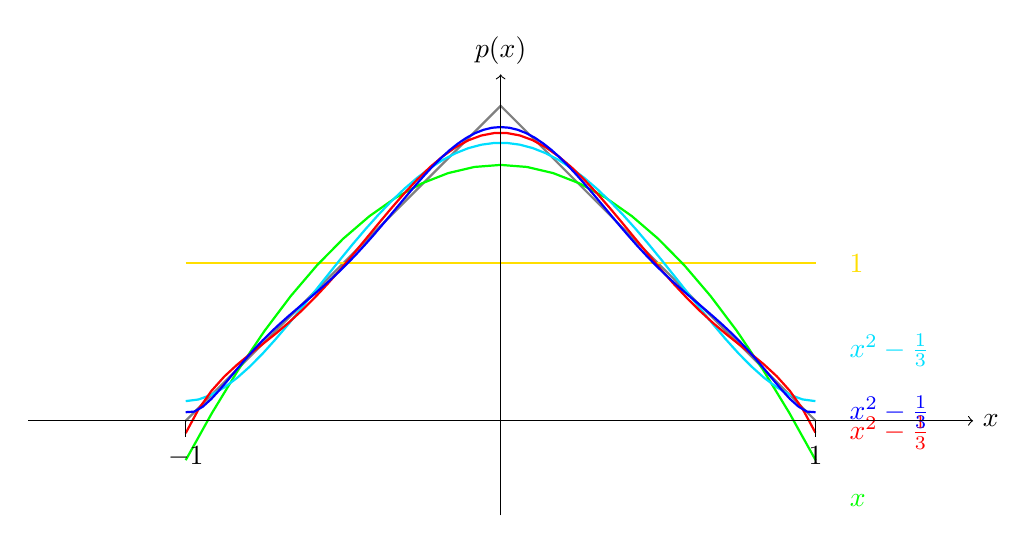
\begin{tikzpicture}[domain=-1:1, scale=4, samples=25]
    \def\fA#1{1}
    \def\fB#1{(#1)}
    \def\fC#1{(abs((#1)^2)-1/3)}
    \def\fD#1{((#1)^3-3/5*(#1))}
    \def\fE#1{(abs((#1)^4)-6/7*abs((#1)^2)+3/35)}
    \def\fF#1{((#1)^5 - 10/9*(#1)^3+5/21*(#1))}
    \def\fG#1{(abs((#1)^6)-15/11*abs((#1)^4)+5/11*abs((#1)^2)-5/231)}
    \def\fH#1{((429*(#1)^7 - 693*(#1)^5 + 315*(#1)^3 - 35*(#1))/429)}
    \def\fI#1{((6435*abs((#1)^8)-12012*abs((#1)^6)+6930*abs((#1)^4)-1260*abs((#1)^2)+35)/6435)}
    \definecolor{my-blue}{rgb}{0,0.87,1.00}
    \definecolor{my-yellow}{rgb}{1.00,0.87,0.00}
    \draw[thick,color=gray] (-1,0) -- (0,1) -- (1,0);
    \draw[thick,color=my-yellow] plot (\x,0.5*\fA{\x}) node[right=2ex] {$1$};
    \draw[thick,color=green] plot (\x,{0.5*\fA{\x} - 0.9375*\fC{\x}}) node[below right=2ex] {$x$};
    \draw[thick,color=my-blue,samples=50] plot (\x,{0.5*\fA{\x} - 0.9375*\fC{\x} + 0.8203125*\fE{\x}}) node[above right=2ex] {$x^2-\frac{1}{3}$};
    \draw[thick,color=red,samples=50] plot (\x,{0.5*\fA{\x} - 0.9375*\fC{\x} + 0.8203125*\fE{\x} -1.46630859375*\fG{\x}}) node[right=2ex] {$x^2-\frac{1}{3}$};
    \draw[thick,color=blue,samples=75] plot (\x,{0.5*\fA{\x} - 0.9375*\fC{\x} + 0.8203125*\fE{\x} -1.46630859375*\fG{\x}+3.338470458984375*\fI{\x}}) node[right=2ex] {$x^2-\frac{1}{3}$};
    \draw[->] (-1.5,0) -- (1.5,0) node[right] {$x$};
    \draw[->] (0,-0.3) -- (0,1.1) node[above] {$p(x)$};
    \draw (1,0) -- (1,-0.05) node[below] {$1$};
    \draw (-1,0) -- (-1,-0.05) node[below] {$-1$};
  \end{tikzpicture}
\end{center}

% ----------------------------------------------------------------------
% Legendre 2

\begin{center}
  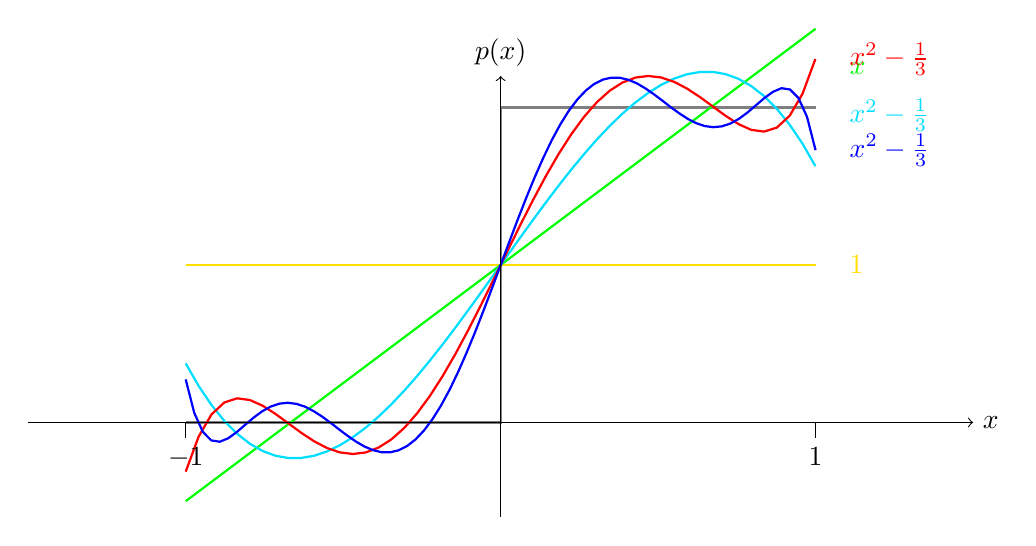
\begin{tikzpicture}[domain=-1:1, scale=4, samples=25]
    \def\fA#1{1}
    \def\fB#1{(#1)}
    \def\fC#1{(abs((#1)^2)-1/3)}
    \def\fD#1{((#1)^3-3/5*(#1))}
    \def\fE#1{(abs((#1)^4)-6/7*abs((#1)^2)+3/35)}
    \def\fF#1{((#1)^5 - 10/9*(#1)^3+5/21*(#1))}
    \def\fG#1{(abs((#1)^6)-15/11*abs((#1)^4)+5/11*abs((#1)^2)-5/231)}
    \def\fH#1{((429*(#1)^7 - 693*(#1)^5 + 315*(#1)^3 - 35*(#1))/429)}
    \def\fI#1{((6435*abs((#1)^8)-12012*abs((#1)^6)+6930*abs((#1)^4)-1260*abs((#1)^2)+35)/6435)}
    \definecolor{my-blue}{rgb}{0,0.87,1.00}
    \definecolor{my-yellow}{rgb}{1.00,0.87,0.00}
    \draw[thick,color=gray] (-1,0) -- (0,0) -- (0,1) -- (1,1);
    \draw[thick,color=my-yellow] plot (\x,0.5*\fA{\x}) node[right=2ex] {$1$};
    \draw[thick,color=green]     plot (\x,{0.5*\fA{\x} + 0.75*\fB{\x}}) node[below right=2ex] {$x$};
    \draw[thick,color=my-blue,samples=50]   plot (\x,{0.5*\fA{\x} + 0.75*\fB{\x} - 1.09375*\fD{\x}}) node[above right=2ex] {$x^2-\frac{1}{3}$};
    \draw[thick,color=red,samples=50]       plot (\x,{0.5*\fA{\x} + 0.75*\fB{\x} - 1.09375*\fD{\x} + 2.70703125*\fF{\x}}) node[right=2ex] {$x^2-\frac{1}{3}$};
    \draw[thick,color=blue,samples=75]      plot (\x,{0.5*\fA{\x} + 0.75*\fB{\x} - 1.09375*\fD{\x} + 2.70703125*\fF{\x} - 7.855224609375*\fH{\x}}) node[right=2ex] {$x^2-\frac{1}{3}$};
    \draw[->] (-1.5,0) -- (1.5,0) node[right] {$x$};
    \draw[->] (0,-0.3) -- (0,1.1) node[above] {$p(x)$};
    \draw (1,0) -- (1,-0.05) node[below] {$1$};
    \draw (-1,0) -- (-1,-0.05) node[below] {$-1$};
  \end{tikzpicture}
\end{center}

% ----------------------------------------------------------------------
% Legendre 3

\begin{center}
  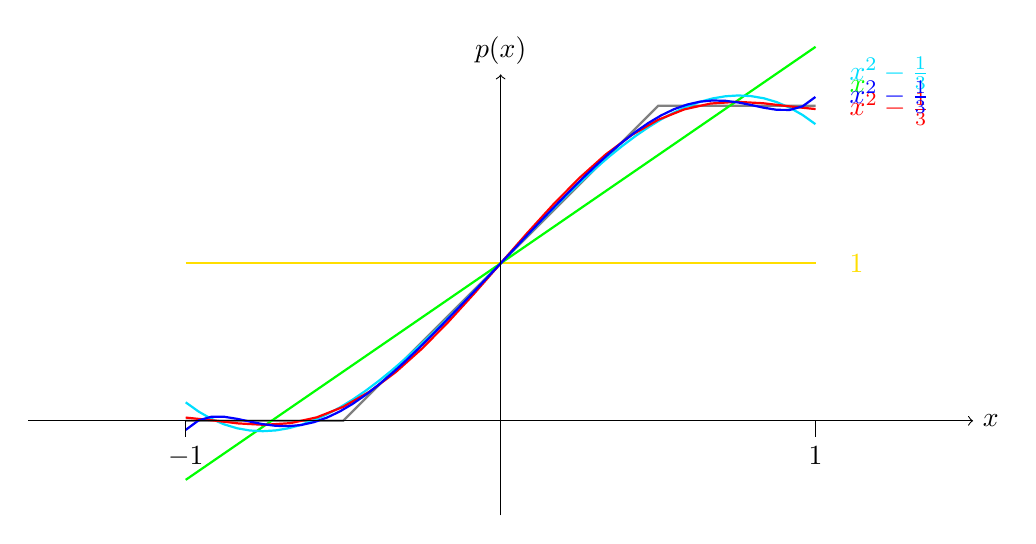
\begin{tikzpicture}[domain=-1:1, scale=4, samples=25]
    \def\fA#1{1}
    \def\fB#1{(#1)}
    \def\fC#1{(abs((#1)^2)-1/3)}
    \def\fD#1{((#1)^3-3/5*(#1))}
    \def\fE#1{(abs((#1)^4)-6/7*abs((#1)^2)+3/35)}
    \def\fF#1{((#1)^5 - 10/9*(#1)^3+5/21*(#1))}
    \def\fG#1{(abs((#1)^6)-15/11*abs((#1)^4)+5/11*abs((#1)^2)-5/231)}
    \def\fH#1{((429*(#1)^7 - 693*(#1)^5 + 315*(#1)^3 - 35*(#1))/429)}
    \def\fI#1{((6435*abs((#1)^8)-12012*abs((#1)^6)+6930*abs((#1)^4)-1260*abs((#1)^2)+35)/6435)}
    \definecolor{my-blue}{rgb}{0,0.87,1.00}
    \definecolor{my-yellow}{rgb}{1.00,0.87,0.00}
    \draw[thick,color=gray] (-1,0) -- (-0.5,0) -- (0.5,1) -- (1,1);
    \draw[thick,color=my-yellow] plot (\x,0.5*\fA{\x}) node[right=2ex] {$1$};
    \draw[thick,color=green]     plot (\x,{0.5*\fA{\x} + 0.6875*\fB{\x}}) node[below right=2ex] {$x$};
    \draw[thick,color=my-blue,samples=50]   plot (\x,{0.5*\fA{\x} + 0.6875*\fB{\x} - 0.615234375*\fD{\x}}) node[above right=2ex] {$x^2-\frac{1}{3}$};
    \draw[thick,color=red]       plot (\x,{0.5*\fA{\x} + 0.6875*\fB{\x} - 0.615234375*\fD{\x} + 0.38067626953125*\fF{\x}}) node[right=2ex] {$x^2-\frac{1}{3}$};
    \draw[thick,color=blue,samples=50]      plot (\x,{0.5*\fA{\x} + 0.6875*\fB{\x} - 0.615234375*\fD{\x} + 0.38067626953125*\fF{\x} + 1.0494089126587303*\fH{\x}}) node[right=2ex] {$x^2-\frac{1}{3}$};
    \draw[->] (-1.5,0) -- (1.5,0) node[right] {$x$};
    \draw[->] (0,-0.3) -- (0,1.1) node[above] {$p(x)$};
    \draw (1,0) -- (1,-0.05) node[below] {$1$};
    \draw (-1,0) -- (-1,-0.05) node[below] {$-1$};
  \end{tikzpicture}
\end{center}

% ----------------------------------------------------------------------
% Fourier 1

\begin{center}
  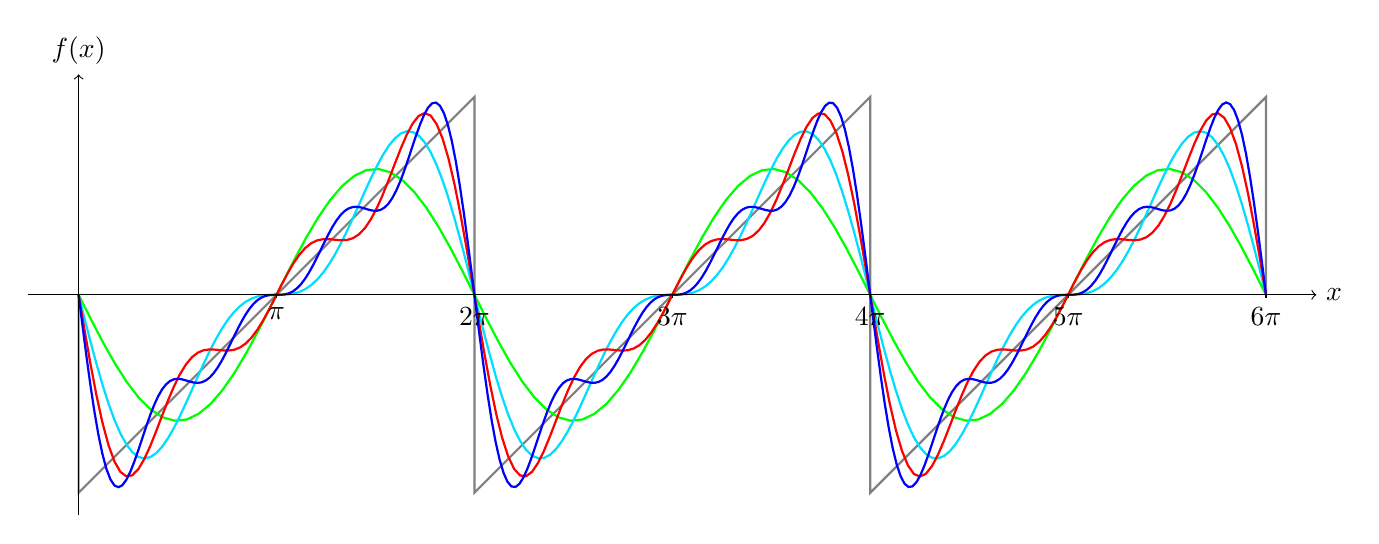
\begin{tikzpicture}[domain=0:6*pi, scale=0.8, samples=100]
    \def\fA#1{1}
    \def\fB#1{(sin((#1)/pi*180)}
    \def\fC#1{(cos((#1)/pi*180))}
    \def\fD#1{(sin(2*(#1)/pi*180))}
    \def\fE#1{(cos(2*(#1)/pi*180))}
    \def\fF#1{(sin(3*(#1)/pi*180))}
    \def\fG#1{(cos(3*(#1)/pi*180))}
    \def\fH#1{(sin(4*(#1)/pi*180))}
    \def\fI#1{(cos(4*(#1)/pi*180))}
    \definecolor{my-blue}{rgb}{0,0.87,1.00}
    \definecolor{my-yellow}{rgb}{1.00,0.87,0.00}
    \draw[thick,color=gray] (0,0) -- (0,-pi) -- (2*pi,pi) -- (2*pi,-pi) --
    (4*pi,pi) -- (4*pi,-pi) -- (6*pi, pi) -- (6*pi, 0);
    \draw[thick,color=green]   plot (\x,{((-2)*\fB{\x})}) node[below right=2ex] {};
    \draw[thick,color=my-blue,samples=200] plot (\x,{((-2)*\fB{\x})+((-1)*\fD{\x})}) node[above right=2ex] {};
    \draw[thick,color=red,samples=200]     plot (\x,{((-2)*\fB{\x})+((-1)*\fD{\x})+((-2/3)*\fF{\x})}) node[right=2ex] {};
    \draw[thick,color=blue,samples=300]    plot (\x,{((-2)*\fB{\x})+((-1)*\fD{\x})+((-2/3)*\fF{\x})+((-1/2)*\fH{\x})}) node[right=2ex] {};
    \draw[->] (-0.8,0) -- (6*pi+0.8,0) node[right] {$x$};
    \draw[->] (0,-3.5) -- (0,3.5) node[above] {$f(x)$};
    \draw (pi,0) -- (pi,-0.05) node[below] {$\pi$};
    \draw (2*pi,0) -- (2*pi,-0.05) node[below] {$2\pi$};
    \draw (3*pi,0) -- (3*pi,-0.05) node[below] {$3\pi$};
    \draw (4*pi,0) -- (4*pi,-0.05) node[below] {$4\pi$};
    \draw (5*pi,0) -- (5*pi,-0.05) node[below] {$5\pi$};
    \draw (6*pi,0) -- (6*pi,-0.05) node[below] {$6\pi$};
  \end{tikzpicture}
\end{center}

\begin{center}
  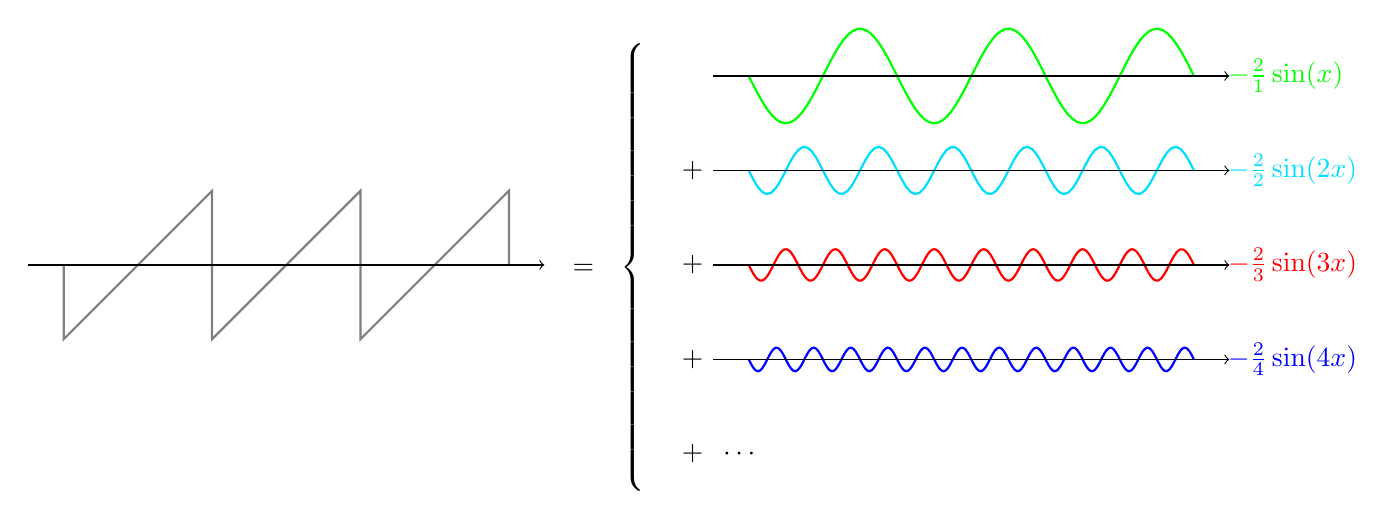
\begin{tikzpicture}[domain=0:6*pi, scale=0.3, samples=100]
    \def\fA#1{1}
    \def\fB#1{(sin((#1)/pi*180)}
    \def\fC#1{(cos((#1)/pi*180))}
    \def\fD#1{(sin(2*(#1)/pi*180))}
    \def\fE#1{(cos(2*(#1)/pi*180))}
    \def\fF#1{(sin(3*(#1)/pi*180))}
    \def\fG#1{(cos(3*(#1)/pi*180))}
    \def\fH#1{(sin(4*(#1)/pi*180))}
    \def\fI#1{(cos(4*(#1)/pi*180))}
    \definecolor{my-blue}{rgb}{0,0.87,1.00}
    \definecolor{my-yellow}{rgb}{1.00,0.87,0.00}
    \begin{scope}[yshift=-12cm,xshift=-29cm]
      \draw[thick,color=gray] (0,0) -- (0,-pi) -- (2*pi,pi) -- (2*pi,-pi) --
      (4*pi,pi) -- (4*pi,-pi) -- (6*pi, pi) -- (6*pi, 0);
      \draw[->] (-1.5,0) -- (6*pi+1.5,0)
      node[right]{$~~=~~\left\{\rule{0mm}{3cm}\right.$};
    \end{scope}
    \begin{scope}[yshift=-4cm]
      \draw[thick,color=green]   plot (\x,{((-2)*\fB{\x})}) node[right=2ex] {$-\frac{2}{1}\sin(x)$};
      \draw[->] (-1.5,0) -- (6*pi+1.5,0);
    \end{scope}
    \begin{scope}[yshift=-8cm]
      \draw[thick,color=my-blue] plot (\x,{((-1)*\fD{\x})}) node[right=2ex] {$-\frac{2}{2}\sin(2x)$};
      \draw[->] (-1.5,0) node[left]{$+$} -- (6*pi+1.5,0);
    \end{scope}
    \begin{scope}[yshift=-12cm]
      \draw[thick,color=red,samples=200]     plot (\x,{((-2/3)*\fF{\x})}) node[right=2ex] {$-\frac{2}{3}\sin(3x)$};
      \draw[->] (-1.5,0) node[left]{$+$} -- (6*pi+1.5,0);
    \end{scope}
    \begin{scope}[yshift=-16cm]
      \draw[thick,color=blue,samples=200]    plot (\x,{((-1/2)*\fH{\x})}) node[right=2ex] {$-\frac{2}{4}\sin(4x)$};
      \draw[->] (-1.5,0) node[left]{$+$} -- (6*pi+1.5,0);
    \end{scope}
    \begin{scope}[yshift=-20cm]
      \path (-1.5,0) node[left]{$+$} node[right]{$\cdots$};
    \end{scope}
  \end{tikzpicture}
\end{center}

% ----------------------------------------------------------------------
% Fourier 2

\begin{center}
  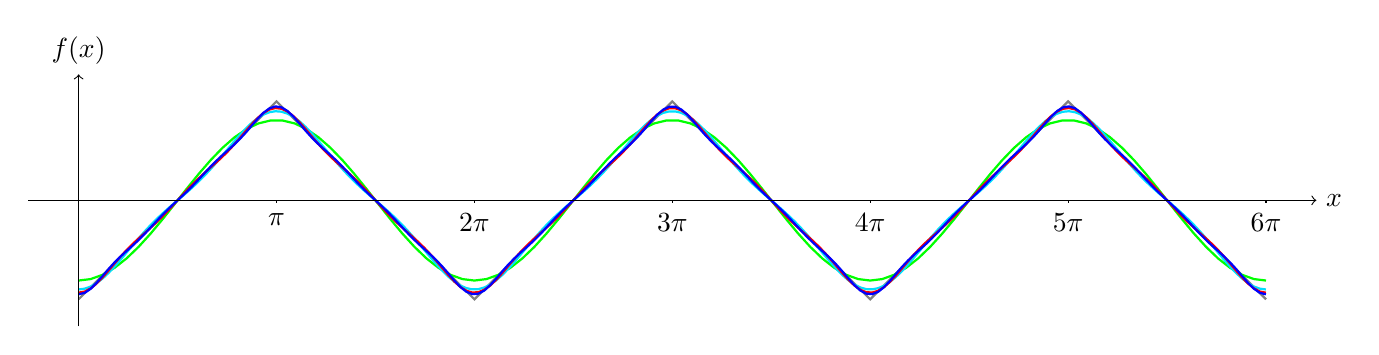
\begin{tikzpicture}[domain=0:6*pi, scale=0.8, samples=100]
    \def\fC#1{(cos((#1)/pi*180))}
    \def\fG#1{(cos(3*(#1)/pi*180))}
    \def\fK#1{(cos(5*(#1)/pi*180))}
    \def\fO#1{(cos(7*(#1)/pi*180))}
    \definecolor{my-blue}{rgb}{0,0.87,1.00}
    \definecolor{my-yellow}{rgb}{1.00,0.87,0.00}
    \draw[thick,color=gray] (0,-pi/2) -- (pi,pi/2) -- (2*pi,-pi/2) -- (3*pi,pi/2) --
    (4*pi,-pi/2) -- (5*pi,pi/2) -- (6*pi, -pi/2);
    \draw[thick,color=green]   plot (\x,{((-1.2732395447351623)*\fC{\x})}) node[below right=2ex] {};
    \draw[thick,color=my-blue,samples=200] plot (\x,{((-1.2732395447351623)*\fC{\x})+((-0.14147106052612904)*\fG{\x})}) node[above right=2ex] {};
    \draw[thick,color=red,samples=200]     plot (\x,{((-1.2732395447351623)*\fC{\x})+((-0.14147106052612904)*\fG{\x})+((-0.05092958178940641)*\fK{\x})}) node[above right=2ex] {};
    \draw[thick,color=blue,samples=200]    plot (\x,{((-1.2732395447351623)*\fC{\x})+((-0.14147106052612904)*\fG{\x})+((-0.05092958178940641)*\fK{\x})+((-0.025984480504798825)*\fO{\x})}) node[above right=2ex] {};
    \draw[->] (-0.8,0) -- (6*pi+0.8,0) node[right] {$x$};
    \draw[->] (0,-2) -- (0,2) node[above] {$f(x)$};
    \draw (pi,0) -- (pi,-0.05) node[below] {$\pi$};
    \draw (2*pi,0) -- (2*pi,-0.05) node[below] {$2\pi$};
    \draw (3*pi,0) -- (3*pi,-0.05) node[below] {$3\pi$};
    \draw (4*pi,0) -- (4*pi,-0.05) node[below] {$4\pi$};
    \draw (5*pi,0) -- (5*pi,-0.05) node[below] {$5\pi$};
    \draw (6*pi,0) -- (6*pi,-0.05) node[below] {$6\pi$};
  \end{tikzpicture}
\end{center}

\begin{center}
  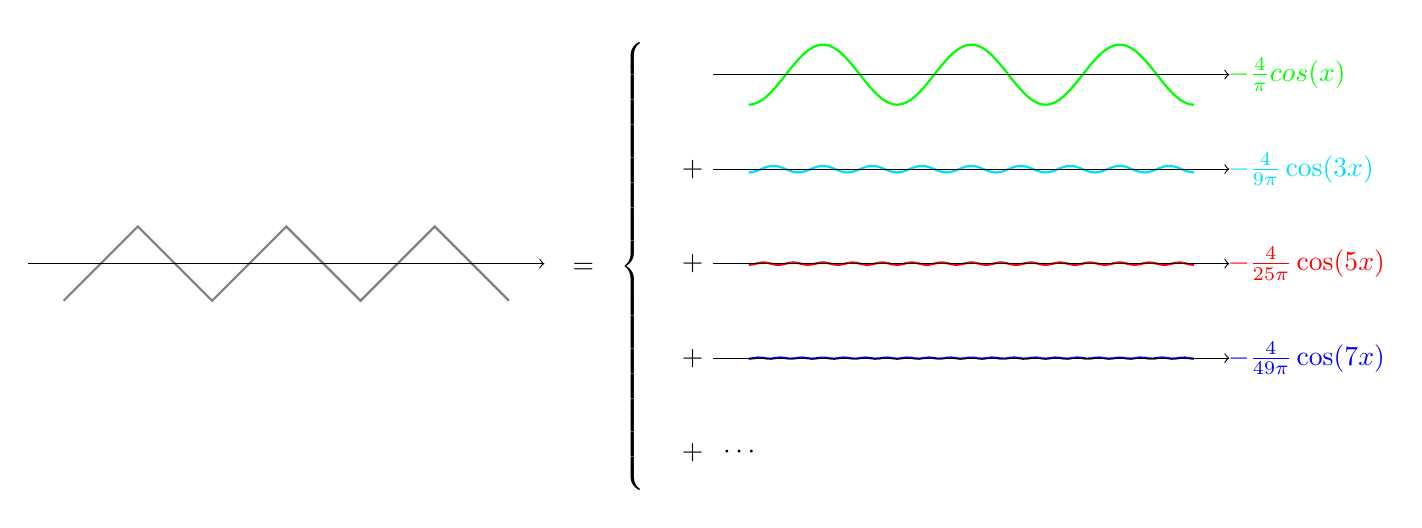
\begin{tikzpicture}[domain=0:6*pi, scale=0.3, samples=100]
    \def\fC#1{(cos((#1)/pi*180))}
    \def\fG#1{(cos(3*(#1)/pi*180))}
    \def\fK#1{(cos(5*(#1)/pi*180))}
    \def\fO#1{(cos(7*(#1)/pi*180))}
    \definecolor{my-blue}{rgb}{0,0.87,1.00}
    \definecolor{my-yellow}{rgb}{1.00,0.87,0.00}
    \begin{scope}[yshift=-12cm,xshift=-29cm]
      \draw[thick,color=gray] (0,-pi/2) -- (pi,pi/2) -- (2*pi,-pi/2) -- (3*pi,pi/2) --
      (4*pi,-pi/2) -- (5*pi,pi/2) -- (6*pi, -pi/2);
      \draw[->] (-1.5,0) -- (6*pi+1.5,0)
      node[right]{$~~=~~\left\{\rule{0mm}{3cm}\right.$};
    \end{scope}
    \begin{scope}[yshift=-4cm]
      \draw[thick,color=green]   plot (\x,{((-1.2732395447351623)*\fC{\x})}) (6*pi,0) node[right=2ex] {$-\frac{4}{\pi}cos(x)$};
      \draw[->] (-1.5,0) -- (6*pi+1.5,0);
    \end{scope}
    \begin{scope}[yshift=-8cm]
      \draw[thick,color=my-blue] plot (\x,{((-0.14147106052612904)*\fG{\x})}) (6*pi,0) node[right=2ex] {$-\frac{4}{9\pi}\cos(3x)$};
      \draw[->] (-1.5,0) node[left]{$+$} -- (6*pi+1.5,0);
    \end{scope}
    \begin{scope}[yshift=-12cm]
      \draw[thick,color=red]     plot (\x,{((-0.05092958178940641)*\fK{\x})}) (6*pi,0) node[right=2ex] {$-\frac{4}{25\pi}\cos(5x)$};
      \draw[->] (-1.5,0) node[left]{$+$} -- (6*pi+1.5,0);
    \end{scope}
    \begin{scope}[yshift=-16cm]
      \draw[thick,color=blue]    plot (\x,{((-0.025984480504798825)*\fO{\x})}) (6*pi,0) node[right=2ex] {$-\frac{4}{49\pi}\cos(7x)$};
      \draw[->] (-1.5,0) node[left]{$+$} -- (6*pi+1.5,0);
    \end{scope}
    \begin{scope}[yshift=-20cm]
      \path (-1.5,0) node[left]{$+$} node[right]{$\cdots$};
    \end{scope}
  \end{tikzpicture}
\end{center}

% ----------------------------------------------------------------------
% Fourier 3

\begin{center}
  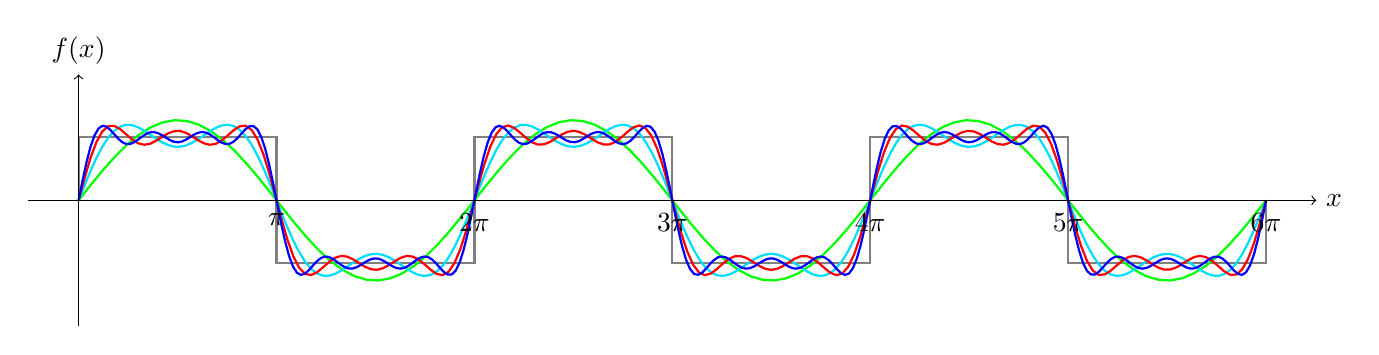
\begin{tikzpicture}[domain=0:6*pi, scale=0.8, samples=100]
    \def\fB#1{(sin((#1)/pi*180))}
    \def\fF#1{(sin(3*(#1)/pi*180))}
    \def\fJ#1{(sin(5*(#1)/pi*180))}
    \def\fN#1{(sin(7*(#1)/pi*180))}
    \definecolor{my-blue}{rgb}{0,0.87,1.00}
    \definecolor{my-yellow}{rgb}{1.00,0.87,0.00}
    \draw[thick,color=gray] (0,0) -- (0,1) -- (pi,1) -- (pi,-1) --
    (2*pi,-1) -- (2*pi,1) --
    (3*pi,1) -- (3*pi,-1) --
    (4*pi,-1) -- (4*pi,1) --
    (5*pi,1) -- (5*pi,-1) --
    (6*pi,-1) -- (6*pi,0);
    \draw[thick,color=green]   plot (\x,{((1.2732395447351623)*\fB{\x})}) node[below right=2ex] {};
    \draw[thick,color=my-blue,samples=200] plot (\x,{((1.2732395447351623)*\fB{\x})+((0.4244131815783881)*\fF{\x})}) node[above right=2ex] {};
    \draw[thick,color=red,samples=200]     plot (\x,{((1.2732395447351623)*\fB{\x})+((0.4244131815783881)*\fF{\x})+((0.25464790894703326)*\fJ{\x})}) node[above right=2ex] {};
    \draw[thick,color=blue,samples=300]    plot (\x,{((1.2732395447351623)*\fB{\x})+((0.4244131815783881)*\fF{\x})+((0.25464790894703326)*\fJ{\x})+((0.18189136353359486)*\fN{\x})}) node[above right=2ex] {};
    \draw[->] (-0.8,0) -- (6*pi+0.8,0) node[right] {$x$};
    \draw[->] (0,-2) -- (0,2) node[above] {$f(x)$};
    \draw (pi,0) -- (pi,-0.05) node[below] {$\pi$};
    \draw (2*pi,0) -- (2*pi,-0.05) node[below] {$2\pi$};
    \draw (3*pi,0) -- (3*pi,-0.05) node[below] {$3\pi$};
    \draw (4*pi,0) -- (4*pi,-0.05) node[below] {$4\pi$};
    \draw (5*pi,0) -- (5*pi,-0.05) node[below] {$5\pi$};
    \draw (6*pi,0) -- (6*pi,-0.05) node[below] {$6\pi$};
  \end{tikzpicture}
\end{center}

\begin{center}
  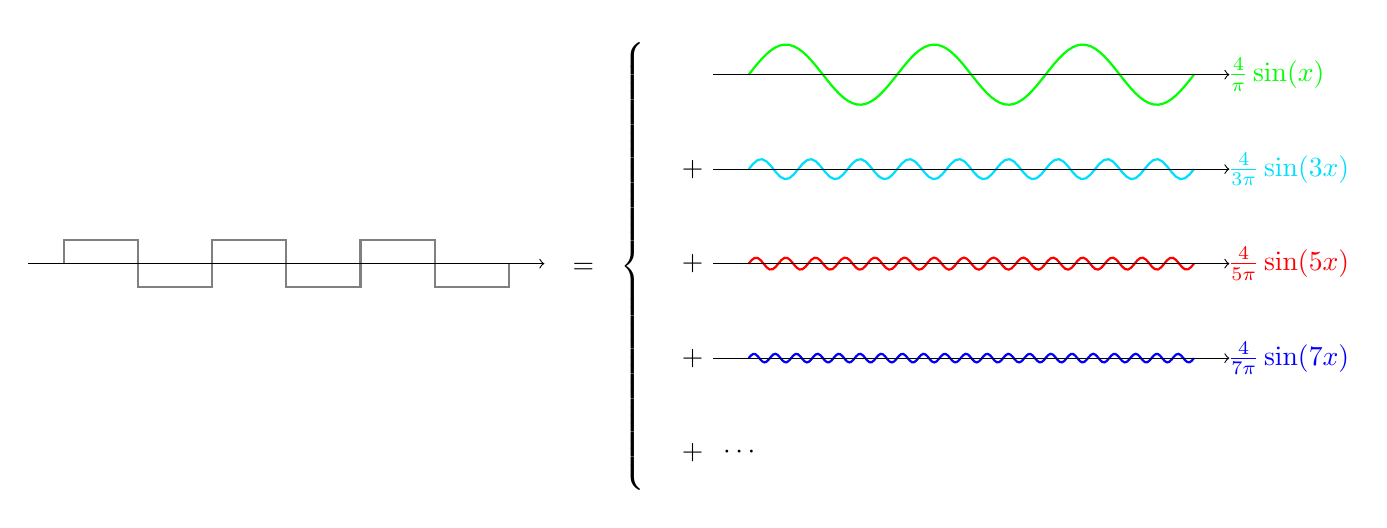
\begin{tikzpicture}[domain=0:6*pi, scale=0.3, samples=100]
    \def\fB#1{(sin((#1)/pi*180))}
    \def\fF#1{(sin(3*(#1)/pi*180))}
    \def\fJ#1{(sin(5*(#1)/pi*180))}
    \def\fN#1{(sin(7*(#1)/pi*180))}
    \definecolor{my-blue}{rgb}{0,0.87,1.00}
    \definecolor{my-yellow}{rgb}{1.00,0.87,0.00}
    \begin{scope}[yshift=-12cm,xshift=-29cm]
      \draw[thick,color=gray] (0,0) -- (0,1) -- (pi,1) -- (pi,-1) --
      (2*pi,-1) -- (2*pi,1) --
      (3*pi,1) -- (3*pi,-1) --
      (4*pi,-1) -- (4*pi,1) --
      (5*pi,1) -- (5*pi,-1) --
      (6*pi,-1) -- (6*pi,0);
      \draw[->] (-1.5,0) -- (6*pi+1.5,0)
      node[right]{$~~=~~\left\{\rule{0mm}{3cm}\right.$};
    \end{scope}
    \begin{scope}[yshift=-4cm]
      \draw[thick,color=green]   plot (\x,{((1.2732395447351623)*\fB{\x})}) node[right=2ex] {$\frac{4}{\pi}\sin(x)$};
      \draw[->] (-1.5,0) -- (6*pi+1.5,0);
    \end{scope}
    \begin{scope}[yshift=-8cm]
      \draw[thick,color=my-blue] plot (\x,{((0.4244131815783881)*\fF{\x})}) node[right=2ex] {$\frac{4}{3\pi}\sin(3x)$};
      \draw[->] (-1.5,0) node[left]{$+$} -- (6*pi+1.5,0);
    \end{scope}
    \begin{scope}[yshift=-12cm]
      \draw[thick,color=red,samples=150]     plot (\x,{((0.25464790894703326)*\fJ{\x})}) node[right=2ex] {$\frac{4}{5\pi}\sin(5x)$};
      \draw[->] (-1.5,0) node[left]{$+$} -- (6*pi+1.5,0);
    \end{scope}
    \begin{scope}[yshift=-16cm]
      \draw[thick,color=blue,samples=200]    plot (\x,{((0.18189136353359486)*\fN{\x})}) node[right=2ex] {$\frac{4}{7\pi}\sin(7x)$};
      \draw[->] (-1.5,0) node[left]{$+$} -- (6*pi+1.5,0);
    \end{scope}
    \begin{scope}[yshift=-20cm]
      \path (-1.5,0) node[left]{$+$} node[right]{$\cdots$};
    \end{scope}
  \end{tikzpicture}
\end{center}
}
